\section{Theorie}

In diesem Versuch wird ein Helium-Neon-Laser (kurz: HeNe-Laser) untersucht.
Laser an sich zeichnen sich dadurch aus, dass sie monochromatisches Licht
mit hoher Intensität und vor allem hoher Kohärenz aussenden. Zu diesem Zweck besteht
der Laser aus drei Komponenten: einem Lasermedium, einer Pumpquelle und einem Resonator.
Mit der Pumpquelle wird eine Besetzungsinversion erzeugt und durch Resonator und Lasermedium
wird ein selbsterregender Oszillator geschaffen. Durch das Lasermedium wird ebenso
das Strahlungsspektrum festgelegt.

Wird ein Zwei-Niveau System mit den Besetzungszahlen $n_1$ (Grundzustand) und
$n_2$ (angeregter Zustand) betrachtet,
dann wird unter Einfall eines Photons, dessen Energie genau der Differenz der beiden
Niveaus entspricht, ein Atom angeregt und geht in den angeregten Zustand über.
Aus diesem geht es entweder durch spontane oder induzierte Emission unter
Aussenden eines Photons wieder in den
Grundzustand über. Schematisch ist das in \autoref{abb:schema_absopr} dargestellt.
\begin{figure}
  \centering
  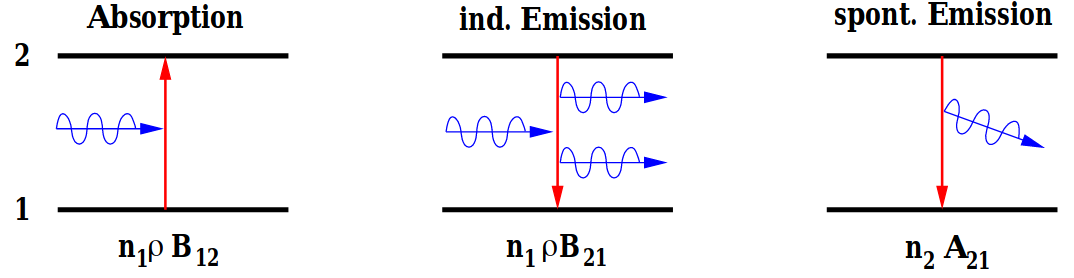
\includegraphics[scale=0.4]{content/pics/schema_absorp.png}
  \caption{Schematische Darstellung des Absorptionsvorgangs und der Emissionsvorgänge
  in einem zwei Niveau-System \cite{anleitung}.}
  \label{abb:schema_absopr}
\end{figure}
Falls das Übergang aus dem angeregten Zustand wieder in den Grundzustand durch ein
einfallendes Photon stimuliert wird, dann hat das emittierte Photon die gleiche Energie,
Phase und Ausbreitungsrichtung wie das Auslöser-Photon. Somit lässt sich festhalten,
dass die Besetzungszahl $n_2$ durch Absorption erhöht und durch die beiden Emissionsarten
verringert wird. Das lässt sich in Formeln gießen:
\begin{align*}
  \dot{N}_A &= n_1 \, \rho(\nu) \, B_{12} &\text{Absorption} \\
  \dot{N}_{IE} &= n_2 \, \rho(\nu) \, B_{21} &\text{induzierte Emission} \\
  \dot{N}_E &= n_2 \, A_{21} &\text{spontane Emission}
\end{align*}
Dabei sind die $\dot{N}_i$ die Anzahl der pro Sekunde und pro Volumeneinheit absorbierten
bzw. emittierten Photonen, $\rho$ die Energiedichte des Strahlungsfeldes und $B_{12}$,
$B_{21}$ und $A_{21}$ Konstanten, die die Übergangwahrscheinlichkeiten angeben.
% Für $n_1 + n_2 = const$ ergibt sich
% \begin{align*}
%   \frac{\symup d n_1}{\symup d t} &= - n_1 \, B_{12} \, \rho + N_2
% \end{align*}
Da im thermischen Gleichgewicht der Grundzustand stärker besetzt ist als der angeregte
Zustand. Um eine dauerhafte Verstärkung des Strahlungsfeldes zu erreichen, muss die
induzierte Emission gegenüber der spontanen Emission überwiegen, indem eine Besetzungsinversion
durchgeführt wird. Diese Verstärkung steigt exponentiell mit der Länge des Lichtlaufweges
an. Um diese Länge zu maximieren, wird der Resonator verwendet, der den Laserstrahl mehrfach
durch das aktive Medium schickt. Dazu werden zwei Spiegel verwendet, einer totalreflexiv
und einer teildurchlässig, damit der Laserstrahl das Gehäuse des Laser verlassen kann.
Da Verluste der Resonatorspiegeln minimiert werden müssen, werden oft konfokale Spiegeln verwendet.
Ein wichtiger Begriff in diesem Zusammenhang ist die optische Stabilität. Diese ist gegeben,
wenn die Verluste im Resonator kleiner sind als die Verstärkung durch die induzierte
Emission. Mit den Resonatorparametern $g_i = 1 - \frac{L}{r_i}$ folgt optische Stabilität,
falls
\begin{equation}
  0 \leq g_1 \cdot g_2 < 1
  \label{eqn:Stabilität}
\end{equation}
erfüllt ist, wobei $L$ die Länge des Resonators und $r_i$ der jeweilige Krümmungsradius
des Spiegels ist.

Viele Wellenlängen können stehende Wellen im Resonator bilden, da im Allgemeinen die
Resonatorlänge sehr viel größer ist als die Wellenlänge des Lasers. Die Anzahl $q$
der verschiedenen Wellenlängen im Resonator heißt longitudinale Mode. Da der Resonator
nicht perfekt ist, gibt es auch transversale Moden. Allgemein werden die Eigenschwingungen
des Resonators $\symup{TEM}_{lpq}$ genannt, mit $l$ bzw. $p$ als Knoten in x- und y-
Richtung. Allgemein haben höhere Moden größere Verluste als niedrige Moden mit höherer
Symmetrie. Die Mode mit der höchsten Symmetrie und den niedrigsten Verlusten ist die
$\symup{TEM}_{00}$ Grundmode, die keine Knoten in transversaler Richtung hat.
Die Intensität dieser Grundmode wird durch eine Gaußverteilung
\begin{equation}
  I(r) = I_0 \exp{\frac{-2 \, r^2}{w^2}}
  \label{eqn:gauß}
\end{equation}
dargestellt, mit $I_0$ als Maximalintensität, $r$ als Abstand zur optischen Achse
und $2 w$ als Strahldurchmesser. Für den Radius des Strahles gilt
\begin{equation}
  w(z) = w_0 \sqrt{1+\left(\frac{\theta \, z}{w_0} \right)^2}
  \label{eqn:radius}
\end{equation}
mit $z$ als Abstand von der minimalen Strahltaille $w_0$ und $\theta = \frac{\lambda}{\pi} \, w_0$
als Strahldivergenz.

Bei dem hier vorliegenden HeNe-Laser wird Helium als Pumpgas und Neon als Lasermedium
verwendet, bei einem Atomverhältnis von 5 zu 1. Mit einem Brewster-Fenster am Ende
des Laserrohrs wird ein möglichst verlustfreier Durchgang von Licht ermöglicht.

\section{Durchführung}
\subsection{Versuchsaufbau}
In \autoref{abb:aufbau} ist ein Foto des experimentellen Aufbaus zu sehen.
\begin{figure}
  \centering
  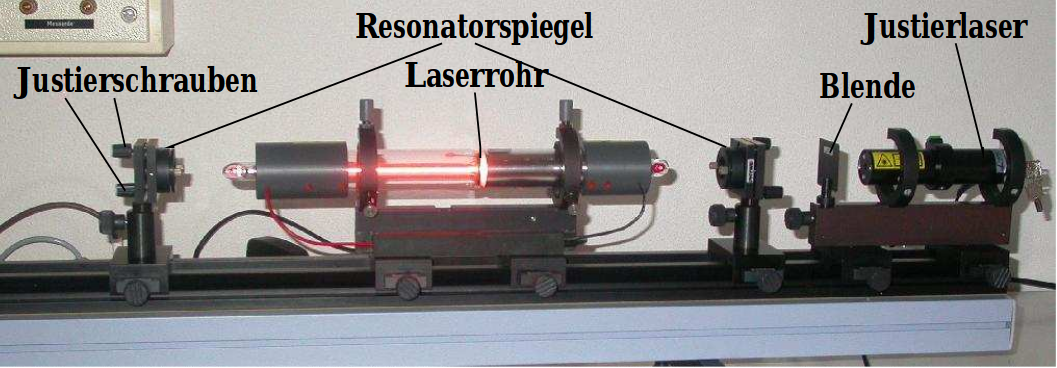
\includegraphics[scale=0.4]{content/pics/aufbau.png}
  \caption{Foto des experimentellen Aufbaus.}
  \label{abb:aufbau}
\end{figure}
Darauf ist ein Justierlaser zu sehen, mit welchem vorjustiert wird. Das Laserrohr
ist mit einem Helium-Neon-Gemisch gefüllt und mit Elektroden versehen. Mit diesen
wird durch elektrische Entladungen die Besetzungsinversion herbeigeführt. Aus vier
verschiedenen Spiegeln kann ausgewählt werden, um einen optischen Resonator aufzubauen.
Außerdem stehen verschiedene optische Geräte zur Verfügung, um die verschiedenen
Eigenschaften des Lasers zu vermessen.

\subsection{Versuchsdurchführung}
Als erstes wird der Lasers mit dem Justierlaser, zwei Schirmen und zwei Blenden
so justiert, dass die Beugungsringe genau auf den auf den Schirmen aufgemalten
Fadenkreuzen liegen. Dies wird jedes Mal überprüft, falls ein neues optisches Element
eingesetzt wird. Als nächstes wird bei maximaler Laserleistung und wechselnden Resonatorabständen
die Stabilitätsbedingung überprüft und die Frequenzen der longitudinalen
Moden gemessen. Außerdem werden mit einem Wolfram-Draht die
TEM-Moden vermessen. Als letztes werden die Polarisation und die Wellenlänge bestimmt.
